\documentclass[10pt,aspectratio=169]{beamer}
\usepackage{tikz}
\usetheme{Boadilla}
\setbeamertemplate{navigation symbols}{}
\title{Incremental analysis: experiments and bounds}
\subtitle{Generated interaction study}
\author{Research group}
\date{}
\year=2026\month=11\day=5
\newcommand{\fuzzlayerA}[1]{\textbf{#1}}
\newcommand{\fuzzlayerB}[1]{\fuzzlayerA{#1}}
\newcommand{\fuzzlayerC}[1]{\fuzzlayerB{#1}}
\newcommand{\fuzzterm}[1]{\fuzzlayerC{#1}}
\newcommand{\fuzzpair}[2]{\fuzzterm{#1}: #2}
\newcommand{\fuzzunit}{ms}
\let\fuzzoriginalunit\fuzzunit
\newcommand{\fuzzcoefficient}{2}
\newcommand{\fuzzscale}[2][\fuzzcoefficient]{#1\,#2}
\definecolor{fuzzpaint}{RGB}{255,0,255}
\definecolor{fuzzsecond}{RGB}{18,137,67}
\tikzset{fuzzvertex/.style={draw,rounded corners=1pt,fill=blue!10,inner sep=1pt,minimum width=.35cm,minimum height=.25cm}}
\begin{document}
\section{Incremental analysis}
\begin{frame}[t,shrink=5]{Incremental analysis}{Composed dependencies}
\fuzzpair{Experiment}{Timing: 12\fuzzunit; estimate $\fuzzscale{x}+\fuzzscale[2]{y}$.}\par
{\renewcommand{\fuzzunit}{samples}\let\fuzzterm\textit\fuzzpair{LocalScope}{Timing: 7\fuzzunit.}\par}
\fuzzpair{RestoredScope}{Timing: 11\fuzzunit.}\par
\begin{columns}[onlytextwidth,b]
\begin{column}{0.54\textwidth}
\begin{itemize}
\item<1-> \begin{enumerate}
\item<1-> \textrm{We compare the} proposed solution with a reference computed from the complete input.  The estimate is $\frac{a+b}{1+c}$.
\item<2-> \begin{enumerate}
\item<1-> \textbf{The final diagram} records the order in which information crosses the partition.  The estimate is $\frac{a+b}{1+c}$.
\item<2-> 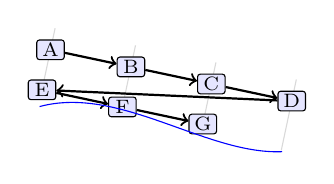
\begin{tikzpicture}[font=\scriptsize]
\begin{scope}[scale=0.8,rotate=-12]

\foreach \x in {0,1,2,3} {\draw[gray!30] (\x*1.305,-.8)--(\x*1.305,.35);}
\node[fuzzvertex] (g6n0) at (0.000,0) {A};
\node[fuzzvertex] (g6n1) at (1.305,0) {B};
\node[fuzzvertex] (g6n2) at (2.610,0) {C};
\node[fuzzvertex] (g6n3) at (3.915,0) {D};
\node[fuzzvertex] (g6n4) at (0.000,-0.65) {E};
\node[fuzzvertex] (g6n5) at (1.305,-0.65) {F};
\node[fuzzvertex] (g6n6) at (2.610,-0.65) {G};
\begin{scope}[xshift=.5pt,yshift=-.5pt]
\draw<2->[->,thick] (g6n0) -- (g6n1);
\draw<2->[->,thick] (g6n1) -- (g6n2);
\draw<2->[->,thick] (g6n2) -- (g6n3);
\draw<2->[->,thick] (g6n3) -- (g6n4);
\draw<2->[->,thick] (g6n4) -- (g6n5);
\draw<2->[->,thick] (g6n5) -- (g6n6);
\draw[blue] (0,-.9) .. controls (1.175,-.3) and (2.741,-1.1) .. (3.915,-.8);
\end{scope}
\end{scope}
\end{tikzpicture}
\end{enumerate}
\end{enumerate}
\item<2-> \begin{alertblock}{Cache invalidation}
\begin{center}
\textbf{We compare the} proposed solution with a reference computed from the complete input.  The estimate is $x_i+x_{i+1}$.
\end{center}
\end{alertblock}
\end{itemize}
\end{column}
\begin{column}{0.42\textwidth}
\textbf{A local update} can change the measurements used by several neighboring components. The next pass must preserve the boundary conditions while revisiting dependent values. The estimate is $x_i+x_{i+1}$.
\par
\textit{We compare the} proposed solution with a reference computed from the complete input.  The estimate is $\sum_{i=1}^{n}x_i$.
\par
\[E=\sum_{i=1}^{n}w_i x_i\]
\par
\begin{columns}[onlytextwidth,c]
\begin{column}{0.38\textwidth}
\begin{tabular}{lrr}Method&Cost&Error\\\hline
Cached0&14&21\\
Global1&5&0\\
Global2&27&16\\
\end{tabular}
\end{column}
\begin{column}{0.58\textwidth}
\begin{tabular}{lrr}Method&Cost&Error\\\hline
Global0&15&14\\
Local1&19&17\\
\end{tabular}
\end{column}
\end{columns}
\par
\begin{enumerate}
\item<1-> \[\begin{aligned}a+b&=c\\ d-e&=f\end{aligned}\]
\item<2-> \[\begin{pmatrix}a&b\\c&d\end{pmatrix}\begin{pmatrix}x\\y\end{pmatrix}\]
\item<3-> \[\begin{aligned}a+b&=c\\ d-e&=f\end{aligned}\]
\end{enumerate}
\end{column}
\end{columns}
\par 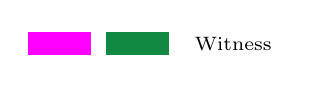
\begin{tikzpicture}[font=\scriptsize]
\fill<2-3>[fuzzpaint] (0,0) rectangle (.8,.3);
\fill<3->[fuzzsecond] (1,0) rectangle (1.8,.3);
\node[anchor=west] at (2,0.15) {Witness};
\end{tikzpicture}
\only<5>{}
\end{frame}
\renewcommand{\fuzzunit}{steps}
\renewcommand{\fuzzcoefficient}{2}
\renewcommand{\fuzzterm}[1]{{\textit{#1}}}
\section{Message passing}
\begin{frame}[t]{Cache invalidation}
\fuzzpair{MacroStageB}{Timing: 12\fuzzunit, retained: 9\fuzzoriginalunit.}\par
{\renewcommand{\fuzzunit}{local}\fuzzpair{FrameLocal}{Timing: 5\fuzzunit.}\par}
\fuzzpair{FrameRestored}{Timing: 8\fuzzunit; estimate $\fuzzscale{x}$.}\par
\begin{columns}[T]\begin{column}{.46\textwidth}The final diagram records the order in which information crosses the partition.\end{column}\begin{column}{.46\textwidth}\begin{itemize}\item Input state\item Updated state\end{itemize}\end{column}\end{columns}
\end{frame}
\renewcommand{\fuzzunit}{Hz}
\renewcommand{\fuzzcoefficient}{3}
\renewcommand{\fuzzterm}[1]{{\textbf{#1}}}
\section{Constraint propagation}
\begin{frame}[t]{Geometric uncertainty}
\fuzzpair{MacroStageC}{Timing: 12\fuzzunit, retained: 9\fuzzoriginalunit.}\par
{\renewcommand{\fuzzunit}{local}\fuzzpair{FrameLocal}{Timing: 5\fuzzunit.}\par}
\fuzzpair{FrameRestored}{Timing: 8\fuzzunit; estimate $\fuzzscale{x}$.}\par
\begin{block}{Follow-up}\fuzzterm{A revised value} depends on the preceding frame.\end{block}
\[r_{k+1}=r_k-\alpha d_k\]
\end{frame}
\renewcommand{\fuzzunit}{steps}
\renewcommand{\fuzzcoefficient}{4}
\renewcommand{\fuzzterm}[1]{{\textrm{#1}}}
\section{Constraint propagation}
\begin{frame}[t]{Cache invalidation}
\fuzzpair{MacroStageD}{Timing: 12\fuzzunit, retained: 9\fuzzoriginalunit.}\par
{\renewcommand{\fuzzunit}{local}\fuzzpair{FrameLocal}{Timing: 5\fuzzunit.}\par}
\fuzzpair{FrameRestored}{Timing: 8\fuzzunit; estimate $\fuzzscale{x}$.}\par
\begin{columns}[T]\begin{column}{.46\textwidth}A narrow column can change line breaking even when the underlying expression is unchanged.\end{column}\begin{column}{.46\textwidth}\begin{itemize}\item Input state\item Updated state\end{itemize}\end{column}\end{columns}
\end{frame}
\end{document}
